%%%%%%%%%%%%%%%%%%%%%%%%%%%%%%%%%%%%%%%%%%%%%%%%%%%%%%%%%%%%%%%%%%% 
%                                                                 %
%                            CHAPTER                              %
%                                                                 %
%%%%%%%%%%%%%%%%%%%%%%%%%%%%%%%%%%%%%%%%%%%%%%%%%%%%%%%%%%%%%%%%%%% 

\chapter{Achtergrond}

\section{Fitnesstrackers}
Zoals al enkele malen werd aangehaald ligt de focus van deze scriptie op
mogelijke tekortkomingen/vulnerabilities betreffende privacybeleid in
fitnesstrackers. Maar voordat een aanval op deze kwetsbaarheden kan worden
opgezet, is het noodzakelijk om een te vat te krijgen op welke manier een
fitnesstracker info verzamelt en weergeeft, en meer precies, hoe de mechanismen
die de privacy voorzien voor de gebruikers in detail werken. Dit is essentiële
informatie om een aanval te kunnen opzetten.

De gebruikte data waarop de aanval wordt opgezet en waar op wordt
geëxperimenteerd, is afkomstig van de populaire fitnesstracker
\textit{Strava\footnote{\url{https://www.strava.com/}}}. Dit is een sociaal
netwerk, waarbij een alle soorten sporters hun activiteiten kunnen delen. Dit
gaat over lopen, wandelen, fietsen, zwemmen, \ldots, maar ook sporten als
fitnessen, voetballen, \ldots (Deze laatste zijn wel veruit in de minderheid
bij het overschouwen van de totale verdeling van alle
activiteiten\cite{Stravas24:online}). De betreffende data wordt in perspectief
van een mogelijke aanval gefilterd, opdat enkel activiteiten die relevante
gps-informatie bevatten in beschouwing worden genomen. Dit gaat dan meer
specifiek over \textit{runs, hikes, walks, and rides}.

\subsection{Activiteiten}\label{data}
Een Strava activiteit bevat erg veel informatie. Echter is niet alles even
bruikbaar. Een correcte abstractie zal dus moeten gemaakt worden van de
onnodige data. Afbeelding~\ref{fig:activityData} geeft een voorbeeld van een
gedetailleerde activiteit weer. Een gebruiker is in staat om de activiteit een
titel te geven, en er een korte beschrijving aan toe te voegen. Ook een foto
kan optioneel toegevoegd worden. De exacte datum en tijd van de start van de
activiteit wordt hierbij ook weergegeven.

Rechts daarvan zijn de algemene basisstatistieken te zien. Deze zijn de totale
afgelegde afstand, de totale bewegingstijd, de gemiddelde snelheid, het totale
hoogteverschil, de totale verstreken tijden het aantal calorieën verbrand. Als
extra kunnen hier enkele statistieken m.b.t.\ het gebruikte materiaal, zoals
type fiets, loopschoenen, hartslagmeter, enzovoort worden weergegeven. Een
belangrijk onderscheid in deze context is het verschil tussen de beweegtijd en
de verstreken tijd. Deze 2 lijken in definitie gelijk, maar dit zijn ze niet!
Strava werkt met 2 verschillende soorten tijdsberekeningen voor een iets
accuratere snelheidsberekening. De verstreken tijd is simpelweg het
tijdsinterval tussen het vertrek van de activiteit en de aankomsttijd ervan. De
bewegingstijd is de tijd waarbij de gebruiker zich effectief bewoog. M.a.w.
worden de tijden waarbij de gebruiker stilstond uit de verstreken tijd
gefilterd. Dit kan gaan over bijvoorbeeld een pauze, of een verkeerslicht. De
snelheid wordt berekend aan de hand van de bewegingstijd. Dit kan simpel worden
geverifieerd worden via een manuele berekening ter bevestiging
(\ref{eq:speed}). Een kanttekening hierbij is dat dit enkel geldt voor
activiteiten die niet gelabeld zijn als \textit{race}. In dit geval wordt de
snelheid berekend in functie van de totaal verstreken
tijd.\cite{MovingTi80:online}
\begin{equation}\label{eq:speed}
    \frac{(39:17)\min}{7.44 km} = 5:16 \min
\end{equation}

Daaronder zien we de \textit{Strava-segmenten}. Een Strava-segment is een
specifiek deel van een bepaalde route dat door gebruikers van de sport-app kan
worden gemarkeerd, gedeeld en vergeleken met andere gebruikers. Het segment is
een bepaalde afstand en route, bijvoorbeeld een klim of afdaling, die vaak
wordt beschouwd als een uitdagende of iconische sectie van een bepaalde fiets-
of hardlooproute. Gebruikers van Strava kunnen een segment maken door de begin-
en eindpunten op een kaart aan te geven en een naam en beschrijving toe te
voegen. Zodra het segment is gemaakt, kunnen andere gebruikers het segment
vinden en deelnemen aan een leaderboard, waarop de snelste tijden worden
bijgehouden en vergeleken met andere gebruikers. Segmenten worden vaak gebruikt
om prestaties te meten en te vergelijken.

Daarnaast is ook de kaart duidelijk zichtbaar. Daarbij horen ook de
tussentijden en de grafiek van snelheid. Optioneel kan hierbij ook nog een
grafiek van de afgelegde hoogte en de hartslag worden weergegeven, indien de
gebruiker hiervoor met het juiste materieel zijn sportactiviteit opneemt. De
tussentijden en de grafiek van snelheid zijn qua inhoud gelijkaardig, met als
verschil dat de grafiek erg precies kan worden bestudeerd worden. Op de grafiek
is voor elk afstandspunt de ogenblikkelijke snelheid zichtbaar. Bij de
tussentijden is wordt de gemiddelde snelheid over een kilometer weergegeven. De
kaart die de route weergeeft is zeker ook belangrijk om even te bestuderen.
Deze bevat namelijk alle gps-geregistreerde punten, en verbindt deze ook om zo
één aaneensluitende route te vormen. Wanneer deze echter in detail bestudeerd
wordt, samen met de legende die aanwezig is, is te zien dat de route uit twee
delen bestaat, een zichtbaar deel en een onzichtbaar deel. Dit heeft betrekking
tot wat zichtbaar is voor een andere gebruiker die deze activiteit bekijkt.
Deze gebruiker zal enkel zicht hebben tot de het zichtbare deel, het
onzichtbare deel zal dus voor een andere gebruiker niet zichtbaar zijn. De
activiteit zal voor deze persoon dus als het ware afgekapt zijn, en zal in zijn
zichtbare versie op een andere plek starten en eindigen. In de volgende
secties~\ref{Algemene Privacy} \&~\ref{EPZ} wordt op de betekenis meer in
detail ingegaan op de werking van deze methodiek.

Een laatste kanttekening die hierbij gemaakt moet worden is dat voor een
gebruiker verschillende eenheden mogelijk zijn om uit te kiezen. Er is keuze
mogelijk tussen de mijl en pond, en kilometer en kilogram. Een gebruiker kiest
in welke eenheid hij/zij de applicatie wenst te gebruiken. Voor de gebruiker in
kwestie zal dus de volledige applicatie worden weergegeven in de gekozen
eenheden.
\begin{figure}
    \centering
    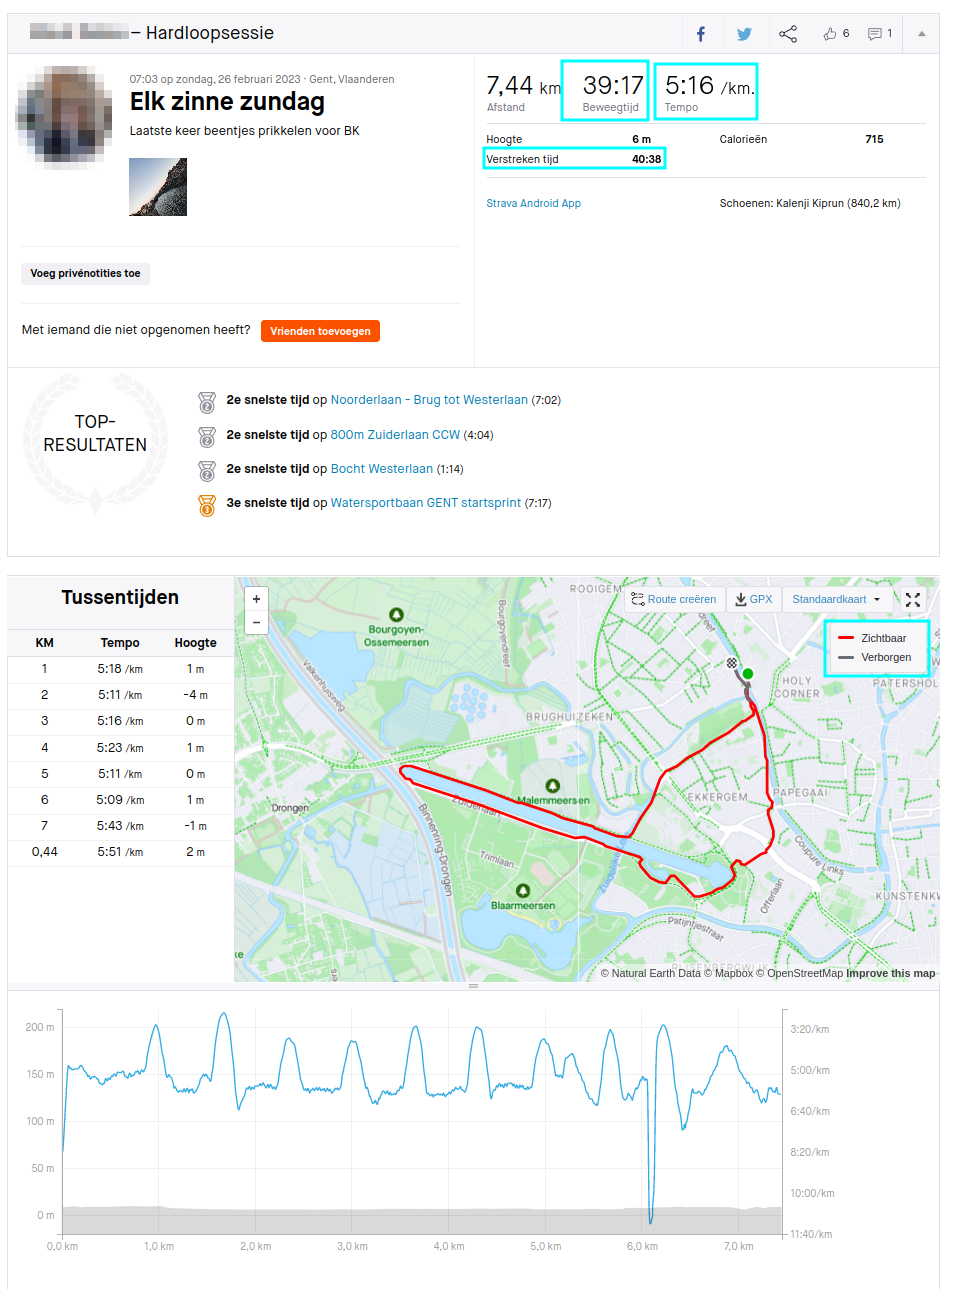
\includegraphics[width=0.8\textwidth]{fig/VoorbeeldActiviteit_Personal.png}
    \caption{Data van een activiteit}\label{fig:activityData}
\end{figure}

\subsection{Berekening Afstanden}
Fitnesstrackers krijgen vanuit de buitenwereld ruwe data binnen. Deze data moet
dus vooraleer ze bruikbaar is voor de gebruiker verwerkt worden. Er werd al
kort ingegaan in sectie~\ref{data} op de berekening die Strava gebruikt voor de
snelheid. Echter is het ook interessant om de berekening van Strava eens onder
de loep te nemen voor de afgelegde afstand. Strava gebruikt 2 aanpakken voor
het berekenen van deze afstand. De eerste is de \textit{GPS-calculated
    Distance}. Dit bestaat eruit om de afstand tussen opeenvolgende punten
gps-punten te berekenen, en deze op te tellen. Precisie is hier afhankelijk van
de precisie van de gps-punten, aangezien de afstand wordt berekend door de
punten te met rechte lijnen te verbinden. Dit kan gebeuren in real time, via
het apparaat die gebruikt wordt om de activiteit op te nemen. In dit geval zal
dit apparaat de cumulatieve afstand berekenen in real time. Op elk punt zal de
afstand vanaf het startpunt gekend zijn, en het is deze afstand die gedeeld zal
worden op het platform. Het grote nadeel hierbij is het real-time aspect.
Fouten kunnen moeilijker on the fly worden gecorrigeerd. Een tweede aanpak is
om het pas bij het uploaden te verwerken. De gps-data wordt dan geanalyseerd,
en de nodige berekeningen kunnen worden uitgevoerd.

Het alternatief voor de GPS-calculated distance is de \textit{Ground Speed
    Distance} methodiek. Deze afstand kan enkel worden bepaald in het geval van een
fietsactiviteit. Deze afstand wordt berekend door het aantal omwentelingen te
vermenigvuldigen met de omtrek van het fietswiel.~\cite{HowDista47:online}
%  Aanvullen... - https://support.strava.com/hc/en-us/articles/216917707-Bad-GPS-Data

\subsection{Algemeen Privacybeleid}\label{Algemene Privacy}
Het delen van alle data die vervat zit in zo'n een activiteit zit met alle
andere gebruikers op het platform, is zeker niet altijd wenselijk. Kiezen er
dan ook voor om de gebruiker de mogelijkheid te geven om zijn privacy te
verbeteren. In deze sectie wordt de focus gelegd op de mechanismen in gebruikt
in \textit{Strava}, maar in heel wat andere sport-applicaties worden
vergelijkbare, zo niet dezelfde methodieken gebruikt. Een eerste algemene
mechanisme bestaat eruit om de gebruiker de keuze te geven om alle activiteiten
en alle gegevens over het profiel heen te laten voldoen aan bepaalde privacy
regels. Deze regels kunnen ook per activiteit worden ingesteld. Onder de keuzes
staan meestal drie opties, \textit{zichtbaar voor iedereen}, \textit{zichtbaar
    voor volgers} en \textit{niemand}. Er kan ook zelf een keuze gemaakt worden om
specifieke elementen van een activiteit niet te delen met de buitenwereld,
zoals bijvoorbeeld de zichtbaarheid van de kaart die de route
weergeeft.\cite{Activity24:online}

\section{Endpoint Privacy Zones}\label{EPZ}
Een tweede significante privacy maatregel is het gebruik van de de
\textbf{Strava Endpoint Privacy Zones (EPZ)}. Deze werden beschreven in een
paper van~\citeauthor{sec18has3:online}. Echter diegene
die~\citeauthor{sec18has3:online} omschreef voldeed niet aan hetgeen in de
praktijk werd waargenomen. Later werd eenzelfde mechanisme omschreven
door~\citeauthor{Dhondt_Pochat_Voulimeneas_Joosen_Volckaert_2022}, die voor
deze omschrijving verder bouwde op de methodiek
van~\citeauthor{sec18has3:online}. Dit is de methodiek die bestudeert en
omzeild wordt in de beide papers, als in de thesis
van~\citeauthor{Verdonck_2022}. Ook in deze thesis wordt een poging gedaan om
de EPZ te omzeilen.

Een EPZ is een cirkelzone met een bepaalde straal rond een gps-punt. De straal
van deze cirkel\footnote{Op Strava heeft de EPZ de vorm van een cirkel, maar op
    andere platformen kunnen andere vormen de norm zijn, bv.\ polygonen.} kan
worden gekozen door de gebruiker, en deze heeft keuze uit waarden van 0 tot
1600m, in stappen van 200m. Wanneer een gebruiker binnen deze zone zijn
activiteit beëindigt of begint, dan de route binnen de EPZ van die activiteit
niet zichtbaar voor andere zijn. Vanuit het perspectief van een andere
gebruiker zal de activiteit dus starten/eindigen op de rand van deze cirkel
(die natuurlijk niet zichtbaar is). Merk op dat een sporter ook andere
gevoelige locaties kan verbergen op de kaart. Dit bij wijze van voorbeeld gaan
over een frequent bezocht café, of een huis van een partner waar regelmatig een
tussenstop plaatsvindt. Een tweede opmerking is dat wanneer een gebruiker de
EPZ doorkruist, maar er niet in stopt, dan zal de route onaangetast blijven. Op
het voorbeeld~\ref{fig:EPZ_Voorbeeld} zijn de verschillende perspectieven te
zien, hoe het er als sporter uitziet, en hoe het eruit ziet volgens een andere
gebruiker. Het traject die de buitenstaander te zien krijgt zijn alle punten
die zich buiten de EPZ bevinden. Merk ook op dat eigenaar van de activiteit
zicht heeft op de EPZ, en wat zal verborgen worden die zich buiten de EPZ
bevinden. Merk ook op dat eigenaar van de activiteit zicht heeft op het effect
van de EPZ, m.a.w.\ welke punten de EPZ zal verbergen. Dit onderscheid wordt
gemaakt door het verschil in kleur (oranje voor de publiek zichtbare punten en
grijs voor de onzichtbare).
\begin{figure}
    \centering
    \begin{subfigure}[b]{.5\textwidth}
        \centering
        \caption{Perspectief eigenaar}
        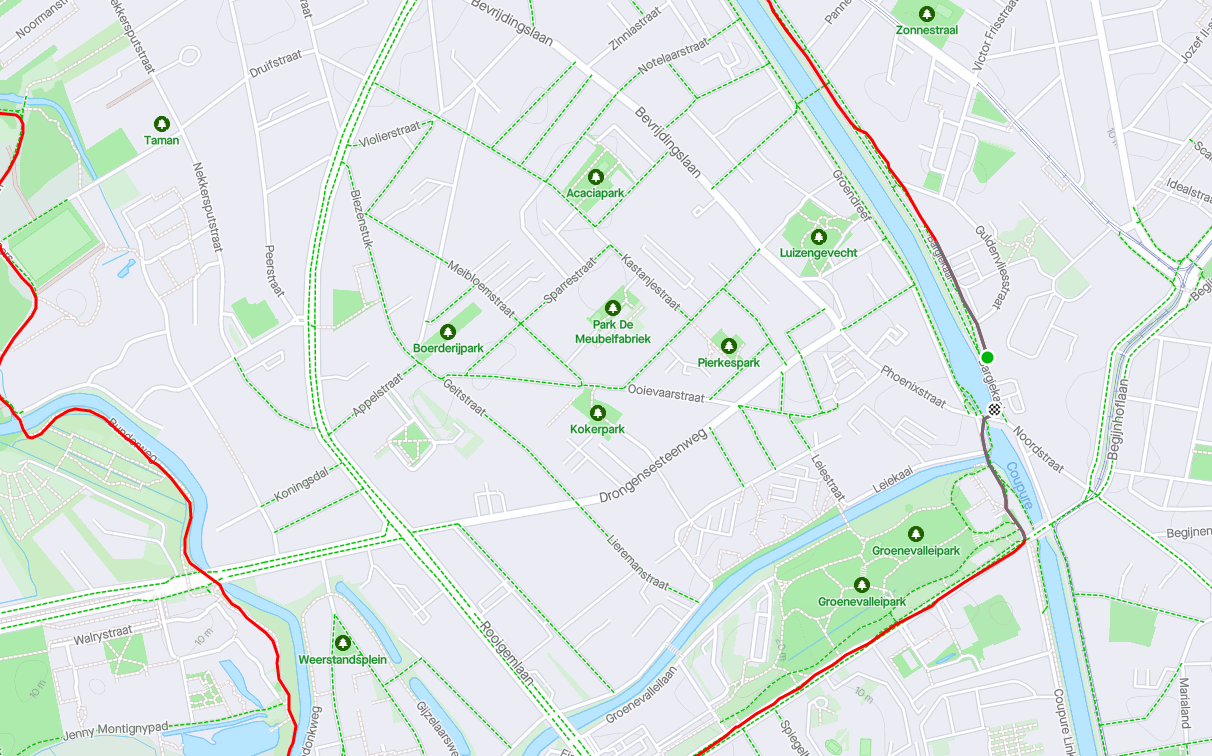
\includegraphics[width=0.8\textwidth]{fig/EPZ_InternalView.png}\label{fig:EPZ_internal}
    \end{subfigure}\hfill
    \begin{subfigure}[b]{.5\textwidth}
        \centering
        \caption{Perspectief externe gebruiker}
        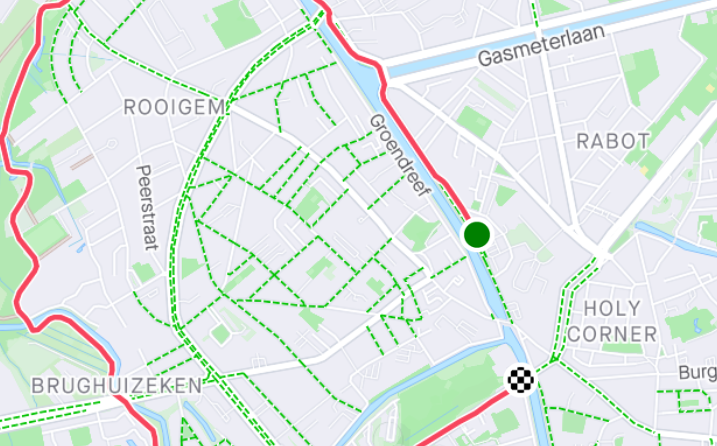
\includegraphics[width=0.8\textwidth]{fig/EPZ_ExternalView.png}\label{fig:EPZ_external}
    \end{subfigure}
    \caption{Voorbeeld van de werking van een EPZ}\label{fig:EPZ_Voorbeeld}
\end{figure}

% Aanvullen
% Uitschrijven smoothing ... Strava
% https://taylor.callsen.me/improving-the-quality-of-gps-track-data/
%https://support.strava.com/hc/en-us/articles/216917707-Bad-GPS-Data